\documentclass[1p]{elsarticle_modified}
%\bibliographystyle{elsarticle-num}

%\usepackage[colorlinks]{hyperref}
%\usepackage{abbrmath_seonhwa} %\Abb, \Ascr, \Acal ,\Abf, \Afrak
\usepackage{amsfonts}
\usepackage{amssymb}
\usepackage{amsmath}
\usepackage{amsthm}
\usepackage{scalefnt}
\usepackage{amsbsy}
\usepackage{kotex}
\usepackage{caption}
\usepackage{subfig}
\usepackage{color}
\usepackage{graphicx}
\usepackage{xcolor} %% white, black, red, green, blue, cyan, magenta, yellow
\usepackage{float}
\usepackage{setspace}
\usepackage{hyperref}

\usepackage{tikz}
\usetikzlibrary{arrows}

\usepackage{multirow}
\usepackage{array} % fixed length table
\usepackage{hhline}

%%%%%%%%%%%%%%%%%%%%%
\makeatletter
\renewcommand*\env@matrix[1][\arraystretch]{%
	\edef\arraystretch{#1}%
	\hskip -\arraycolsep
	\let\@ifnextchar\new@ifnextchar
	\array{*\c@MaxMatrixCols c}}
\makeatother %https://tex.stackexchange.com/questions/14071/how-can-i-increase-the-line-spacing-in-a-matrix
%%%%%%%%%%%%%%%

\usepackage[normalem]{ulem}

\newcommand{\msout}[1]{\ifmmode\text{\sout{\ensuremath{#1}}}\else\sout{#1}\fi}
%SOURCE: \msout is \stkout macro in https://tex.stackexchange.com/questions/20609/strikeout-in-math-mode

\newcommand{\cancel}[1]{
	\ifmmode
	{\color{red}\msout{#1}}
	\else
	{\color{red}\sout{#1}}
	\fi
}

\newcommand{\add}[1]{
	{\color{blue}\uwave{#1}}
}

\newcommand{\replace}[2]{
	\ifmmode
	{\color{red}\msout{#1}}{\color{blue}\uwave{#2}}
	\else
	{\color{red}\sout{#1}}{\color{blue}\uwave{#2}}
	\fi
}

\newcommand{\Sol}{\mathcal{S}} %segment
\newcommand{\D}{D} %diagram
\newcommand{\A}{\mathcal{A}} %arc


%%%%%%%%%%%%%%%%%%%%%%%%%%%%%5 test

\def\sl{\operatorname{\textup{SL}}(2,\Cbb)}
\def\psl{\operatorname{\textup{PSL}}(2,\Cbb)}
\def\quan{\mkern 1mu \triangleright \mkern 1mu}

\theoremstyle{definition}
\newtheorem{thm}{Theorem}[section]
\newtheorem{prop}[thm]{Proposition}
\newtheorem{lem}[thm]{Lemma}
\newtheorem{ques}[thm]{Question}
\newtheorem{cor}[thm]{Corollary}
\newtheorem{defn}[thm]{Definition}
\newtheorem{exam}[thm]{Example}
\newtheorem{rmk}[thm]{Remark}
\newtheorem{alg}[thm]{Algorithm}

\newcommand{\I}{\sqrt{-1}}
\begin{document}

%\begin{frontmatter}
%
%\title{Boundary parabolic representations of knots up to 8 crossings}
%
%%% Group authors per affiliation:
%\author{Yunhi Cho} 
%\address{Department of Mathematics, University of Seoul, Seoul, Korea}
%\ead{yhcho@uos.ac.kr}
%
%
%\author{Seonhwa Kim} %\fnref{s_kim}}
%\address{Center for Geometry and Physics, Institute for Basic Science, Pohang, 37673, Korea}
%\ead{ryeona17@ibs.re.kr}
%
%\author{Hyuk Kim}
%\address{Department of Mathematical Sciences, Seoul National University, Seoul 08826, Korea}
%\ead{hyukkim@snu.ac.kr}
%
%\author{Seokbeom Yoon}
%\address{Department of Mathematical Sciences, Seoul National University, Seoul, 08826,  Korea}
%\ead{sbyoon15@snu.ac.kr}
%
%\begin{abstract}
%We find all boundary parabolic representation of knots up to 8 crossings.
%
%\end{abstract}
%\begin{keyword}
%    \MSC[2010] 57M25 
%\end{keyword}
%
%\end{frontmatter}

%\linenumbers
%\tableofcontents
%
\newcommand\colored[1]{\textcolor{white}{\rule[-0.35ex]{0.8em}{1.4ex}}\kern-0.8em\color{red} #1}%
%\newcommand\colored[1]{\textcolor{white}{ #1}\kern-2.17ex	\textcolor{white}{ #1}\kern-1.81ex	\textcolor{white}{ #1}\kern-2.15ex\color{red}#1	}

{\Large $\underline{12a_{0369}~(K12a_{0369})}$}

\setlength{\tabcolsep}{10pt}
\renewcommand{\arraystretch}{1.6}
\vspace{1cm}\begin{tabular}{m{100pt}>{\centering\arraybackslash}m{274pt}}
\multirow{5}{120pt}{
	\centering
	\includegraphics[width=112pt]{../../../GIT/diagram.site/Diagrams/png/1170_12a_0369.png}\\
\ \ \ A knot diagram\footnotemark}&
\allowdisplaybreaks
\textbf{Linearized knot diagam} \\
\cline{2-2}
 &
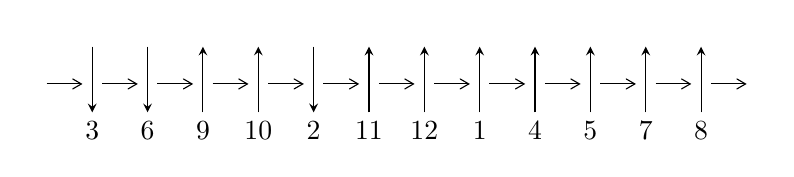
\begin{tikzpicture}[x=20pt, y=17pt]
	% nodes
	\node (C0) at (0, 0) {};
	\node (C1) at (1, 0) {};
	\node (C1U) at (1, +1) {};
	\node (C1D) at (1, -1) {3};

	\node (C2) at (2, 0) {};
	\node (C2U) at (2, +1) {};
	\node (C2D) at (2, -1) {6};

	\node (C3) at (3, 0) {};
	\node (C3U) at (3, +1) {};
	\node (C3D) at (3, -1) {9};

	\node (C4) at (4, 0) {};
	\node (C4U) at (4, +1) {};
	\node (C4D) at (4, -1) {10};

	\node (C5) at (5, 0) {};
	\node (C5U) at (5, +1) {};
	\node (C5D) at (5, -1) {2};

	\node (C6) at (6, 0) {};
	\node (C6U) at (6, +1) {};
	\node (C6D) at (6, -1) {11};

	\node (C7) at (7, 0) {};
	\node (C7U) at (7, +1) {};
	\node (C7D) at (7, -1) {12};

	\node (C8) at (8, 0) {};
	\node (C8U) at (8, +1) {};
	\node (C8D) at (8, -1) {1};

	\node (C9) at (9, 0) {};
	\node (C9U) at (9, +1) {};
	\node (C9D) at (9, -1) {4};

	\node (C10) at (10, 0) {};
	\node (C10U) at (10, +1) {};
	\node (C10D) at (10, -1) {5};

	\node (C11) at (11, 0) {};
	\node (C11U) at (11, +1) {};
	\node (C11D) at (11, -1) {7};

	\node (C12) at (12, 0) {};
	\node (C12U) at (12, +1) {};
	\node (C12D) at (12, -1) {8};
	\node (C13) at (13, 0) {};

	% arrows
	\draw[->,>={angle 60}]
	(C0) edge (C1) (C1) edge (C2) (C2) edge (C3) (C3) edge (C4) (C4) edge (C5) (C5) edge (C6) (C6) edge (C7) (C7) edge (C8) (C8) edge (C9) (C9) edge (C10) (C10) edge (C11) (C11) edge (C12) (C12) edge (C13) ;	\draw[->,>=stealth]
	(C1U) edge (C1D) (C2U) edge (C2D) (C3D) edge (C3U) (C4D) edge (C4U) (C5U) edge (C5D) (C6D) edge (C6U) (C7D) edge (C7U) (C8D) edge (C8U) (C9D) edge (C9U) (C10D) edge (C10U) (C11D) edge (C11U) (C12D) edge (C12U) ;
	\end{tikzpicture} \\
\hhline{~~} \\& 
\textbf{Solving Sequence} \\ \cline{2-2} 
 &
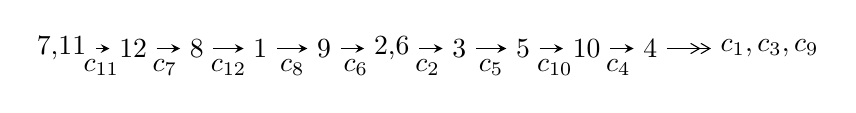
\begin{tikzpicture}[x=23pt, y=7pt]
	% node
	\node (A0) at (-1/8, 0) {7,11};
	\node (A1) at (1, 0) {12};
	\node (A2) at (2, 0) {8};
	\node (A3) at (3, 0) {1};
	\node (A4) at (4, 0) {9};
	\node (A5) at (81/16, 0) {2,6};
	\node (A6) at (49/8, 0) {3};
	\node (A7) at (57/8, 0) {5};
	\node (A8) at (65/8, 0) {10};
	\node (A9) at (73/8, 0) {4};
	\node (C1) at (1/2, -1) {$c_{11}$};
	\node (C2) at (3/2, -1) {$c_{7}$};
	\node (C3) at (5/2, -1) {$c_{12}$};
	\node (C4) at (7/2, -1) {$c_{8}$};
	\node (C5) at (9/2, -1) {$c_{6}$};
	\node (C6) at (45/8, -1) {$c_{2}$};
	\node (C7) at (53/8, -1) {$c_{5}$};
	\node (C8) at (61/8, -1) {$c_{10}$};
	\node (C9) at (69/8, -1) {$c_{4}$};
	\node (A10) at (11, 0) {$c_{1},c_{3},c_{9}$};

	% edge
	\draw[->,>=stealth]	
	(A0) edge (A1) (A1) edge (A2) (A2) edge (A3) (A3) edge (A4) (A4) edge (A5) (A5) edge (A6) (A6) edge (A7) (A7) edge (A8) (A8) edge (A9) ;
	\draw[->>,>={angle 60}]	
	(A9) edge (A10);
\end{tikzpicture} \\ 

\end{tabular} \\

\footnotetext{
The image of knot diagram is generated by the software ``\textbf{Draw programme}" developed by Andrew Bartholomew(\url{http://www.layer8.co.uk/maths/draw/index.htm\#Running-draw}), where we modified some parts for our purpose(\url{https://github.com/CATsTAILs/LinksPainter}).
}\phantom \\ \newline 
\centering \textbf{Ideals for irreducible components\footnotemark of $X_{\text{par}}$} 
 
\begin{align*}
I^u_{1}&=\langle 
-478134295627 u^{38}+149778839704 u^{37}+\cdots+783747150866 b-1669436053919,\\
\phantom{I^u_{1}}&\phantom{= \langle  }-19258298275 u^{38}-10323980760 u^{37}+\cdots+783747150866 a+8187780738725,\\
\phantom{I^u_{1}}&\phantom{= \langle  }u^{39}-2 u^{38}+\cdots+10 u-1\rangle \\
I^u_{2}&=\langle 
b+a+u-1,\;a^2+4 a u-2 a+3,\;u^2- u-1\rangle \\
I^u_{3}&=\langle 
b+u,\;a-2 u-1,\;u^2+u-1\rangle \\
\\
\end{align*}
\raggedright * 3 irreducible components of $\dim_{\mathbb{C}}=0$, with total 45 representations.\\
\footnotetext{All coefficients of polynomials are rational numbers. But the coefficients are sometimes approximated in decimal forms when there is not enough margin.}
\newpage
\renewcommand{\arraystretch}{1}
\centering \section*{I. $I^u_{1}= \langle -4.78\times10^{11} u^{38}+1.50\times10^{11} u^{37}+\cdots+7.84\times10^{11} b-1.67\times10^{12},\;-1.93\times10^{10} u^{38}-1.03\times10^{10} u^{37}+\cdots+7.84\times10^{11} a+8.19\times10^{12},\;u^{39}-2 u^{38}+\cdots+10 u-1 \rangle$}
\flushleft \textbf{(i) Arc colorings}\\
\begin{tabular}{m{7pt} m{180pt} m{7pt} m{180pt} }
\flushright $a_{7}=$&$\begin{pmatrix}0\\u\end{pmatrix}$ \\
\flushright $a_{11}=$&$\begin{pmatrix}1\\0\end{pmatrix}$ \\
\flushright $a_{12}=$&$\begin{pmatrix}1\\- u^2\end{pmatrix}$ \\
\flushright $a_{8}=$&$\begin{pmatrix}u\\- u^3+u\end{pmatrix}$ \\
\flushright $a_{1}=$&$\begin{pmatrix}- u^2+1\\u^4-2 u^2\end{pmatrix}$ \\
\flushright $a_{9}=$&$\begin{pmatrix}- u^3+2 u\\u^5-3 u^3+u\end{pmatrix}$ \\
\flushright $a_{2}=$&$\begin{pmatrix}0.0245721 u^{38}+0.0131726 u^{37}+\cdots-11.4436 u-10.4470\\0.610062 u^{38}-0.191106 u^{37}+\cdots-5.42326 u+2.13007\end{pmatrix}$ \\
\flushright $a_{6}=$&$\begin{pmatrix}- u\\u\end{pmatrix}$ \\
\flushright $a_{3}=$&$\begin{pmatrix}-0.819512 u^{38}+1.59433 u^{37}+\cdots-1.16490 u-11.5383\\1.45415 u^{38}-1.77227 u^{37}+\cdots-15.7020 u+3.22140\end{pmatrix}$ \\
\flushright $a_{5}=$&$\begin{pmatrix}4.72658 u^{38}-5.95208 u^{37}+\cdots-44.4581 u+17.4015\\-2.05862 u^{38}+2.32509 u^{37}+\cdots+22.0842 u-3.94672\end{pmatrix}$ \\
\flushright $a_{10}=$&$\begin{pmatrix}-2.46589 u^{38}+3.88914 u^{37}+\cdots+4.27839 u-17.1124\\-0.582048 u^{38}+0.868548 u^{37}+\cdots+13.4013 u+0.570488\end{pmatrix}$ \\
\flushright $a_{4}=$&$\begin{pmatrix}0.883550 u^{38}-0.877719 u^{37}+\cdots-20.4637 u-8.99829\\1.11038 u^{38}-0.900266 u^{37}+\cdots-10.7236 u+2.76872\end{pmatrix}$\\&\end{tabular}
\flushleft \textbf{(ii) Obstruction class $= -1$}\\~\\
\flushleft \textbf{(iii) Cusp Shapes $= -\frac{627190064793}{391873575433} u^{38}+\frac{1064333701951}{391873575433} u^{37}+\cdots-\frac{1173686425629}{391873575433} u+\frac{611656068405}{391873575433}$}\\~\\
\newpage\renewcommand{\arraystretch}{1}
\flushleft \textbf{(iv) u-Polynomials at the component}\newline \\
\begin{tabular}{m{50pt}|m{274pt}}
Crossings & \hspace{64pt}u-Polynomials at each crossing \\
\hline $$\begin{aligned}c_{1}\end{aligned}$$&$\begin{aligned}
&u^{39}+15 u^{38}+\cdots+111 u+1
\end{aligned}$\\
\hline $$\begin{aligned}c_{2},c_{5}\end{aligned}$$&$\begin{aligned}
&u^{39}+3 u^{38}+\cdots+3 u+1
\end{aligned}$\\
\hline $$\begin{aligned}c_{3},c_{4},c_{9}\\c_{10}\end{aligned}$$&$\begin{aligned}
&u^{39}- u^{38}+\cdots+4 u-4
\end{aligned}$\\
\hline $$\begin{aligned}c_{6},c_{7},c_{8}\\c_{11},c_{12}\end{aligned}$$&$\begin{aligned}
&u^{39}+2 u^{38}+\cdots+10 u+1
\end{aligned}$\\
\hline
\end{tabular}\\~\\
\newpage\renewcommand{\arraystretch}{1}
\flushleft \textbf{(v) Riley Polynomials at the component}\newline \\
\begin{tabular}{m{50pt}|m{274pt}}
Crossings & \hspace{64pt}Riley Polynomials at each crossing \\
\hline $$\begin{aligned}c_{1}\end{aligned}$$&$\begin{aligned}
&y^{39}+25 y^{38}+\cdots+6327 y-1
\end{aligned}$\\
\hline $$\begin{aligned}c_{2},c_{5}\end{aligned}$$&$\begin{aligned}
&y^{39}-15 y^{38}+\cdots+111 y-1
\end{aligned}$\\
\hline $$\begin{aligned}c_{3},c_{4},c_{9}\\c_{10}\end{aligned}$$&$\begin{aligned}
&y^{39}-49 y^{38}+\cdots+368 y-16
\end{aligned}$\\
\hline $$\begin{aligned}c_{6},c_{7},c_{8}\\c_{11},c_{12}\end{aligned}$$&$\begin{aligned}
&y^{39}-54 y^{38}+\cdots+102 y-1
\end{aligned}$\\
\hline
\end{tabular}\\~\\
\newpage\flushleft \textbf{(vi) Complex Volumes and Cusp Shapes}
$$\begin{array}{c|c|c}  
\text{Solutions to }I^u_{1}& \I (\text{vol} + \sqrt{-1}CS) & \text{Cusp shape}\\
 \hline 
\begin{aligned}
u &= -1.020110 + 0.131184 I \\
a &= -1.009270 + 0.527233 I \\
b &= \phantom{-}0.286806 - 1.184210 I\end{aligned}
 & \phantom{-}2.30767 - 2.27298 I & \phantom{-}10.27248 + 3.27626 I \\ \hline\begin{aligned}
u &= -1.020110 - 0.131184 I \\
a &= -1.009270 - 0.527233 I \\
b &= \phantom{-}0.286806 + 1.184210 I\end{aligned}
 & \phantom{-}2.30767 + 2.27298 I & \phantom{-}10.27248 - 3.27626 I \\ \hline\begin{aligned}
u &= -1.04641\phantom{ +0.000000I} \\
a &= \phantom{-}3.22469\phantom{ +0.000000I} \\
b &= -1.92904\phantom{ +0.000000I}\end{aligned}
 & \phantom{-}7.09140\phantom{ +0.000000I} & \phantom{-}13.7060\phantom{ +0.000000I} \\ \hline\begin{aligned}
u &= \phantom{-}1.073560 + 0.109186 I \\
a &= -0.557430 - 0.305343 I \\
b &= -0.051344 - 0.282062 I\end{aligned}
 & \phantom{-}5.55859 + 1.07065 I & \phantom{-}15.4669 - 1.4412 I \\ \hline\begin{aligned}
u &= \phantom{-}1.073560 - 0.109186 I \\
a &= -0.557430 + 0.305343 I \\
b &= -0.051344 + 0.282062 I\end{aligned}
 & \phantom{-}5.55859 - 1.07065 I & \phantom{-}15.4669 + 1.4412 I \\ \hline\begin{aligned}
u &= \phantom{-}1.062930 + 0.284051 I \\
a &= -1.64402 - 0.62028 I \\
b &= \phantom{-}0.93533 + 1.43760 I\end{aligned}
 & \phantom{-}4.46872 + 6.29211 I & \phantom{-}12.7084 - 7.5348 I \\ \hline\begin{aligned}
u &= \phantom{-}1.062930 - 0.284051 I \\
a &= -1.64402 + 0.62028 I \\
b &= \phantom{-}0.93533 - 1.43760 I\end{aligned}
 & \phantom{-}4.46872 - 6.29211 I & \phantom{-}12.7084 + 7.5348 I \\ \hline\begin{aligned}
u &= -1.109570 + 0.405465 I \\
a &= -2.09516 + 0.56202 I \\
b &= \phantom{-}1.43927 - 1.50328 I\end{aligned}
 & \phantom{-}12.9852 - 8.7765 I & \phantom{-}14.1494 + 5.9356 I \\ \hline\begin{aligned}
u &= -1.109570 - 0.405465 I \\
a &= -2.09516 - 0.56202 I \\
b &= \phantom{-}1.43927 + 1.50328 I\end{aligned}
 & \phantom{-}12.9852 + 8.7765 I & \phantom{-}14.1494 - 5.9356 I \\ \hline\begin{aligned}
u &= \phantom{-}0.801500\phantom{ +0.000000I} \\
a &= \phantom{-}2.55587\phantom{ +0.000000I} \\
b &= -1.10388\phantom{ +0.000000I}\end{aligned}
 & -0.106375\phantom{ +0.000000I} & \phantom{-}16.7010\phantom{ +0.000000I}\\
 \hline 
 \end{array}$$\newpage$$\begin{array}{c|c|c}  
\text{Solutions to }I^u_{1}& \I (\text{vol} + \sqrt{-1}CS) & \text{Cusp shape}\\
 \hline 
\begin{aligned}
u &= \phantom{-}0.476965 + 0.626572 I \\
a &= \phantom{-}1.09357 + 0.93891 I \\
b &= \phantom{-}0.323319 - 1.133120 I\end{aligned}
 & \phantom{-}9.07010 - 0.79273 I & \phantom{-}12.42094 - 0.46386 I \\ \hline\begin{aligned}
u &= \phantom{-}0.476965 - 0.626572 I \\
a &= \phantom{-}1.09357 - 0.93891 I \\
b &= \phantom{-}0.323319 + 1.133120 I\end{aligned}
 & \phantom{-}9.07010 + 0.79273 I & \phantom{-}12.42094 + 0.46386 I \\ \hline\begin{aligned}
u &= \phantom{-}0.783899\phantom{ +0.000000I} \\
a &= \phantom{-}0.595351\phantom{ +0.000000I} \\
b &= -1.19130\phantom{ +0.000000I}\end{aligned}
 & \phantom{-}5.58284\phantom{ +0.000000I} & \phantom{-}18.2860\phantom{ +0.000000I} \\ \hline\begin{aligned}
u &= \phantom{-}0.311989 + 0.683555 I \\
a &= \phantom{-}0.474675 - 0.108825 I \\
b &= -0.86174 - 1.47607 I\end{aligned}
 & \phantom{-}8.56307 + 5.06640 I & \phantom{-}11.02566 - 5.09114 I \\ \hline\begin{aligned}
u &= \phantom{-}0.311989 - 0.683555 I \\
a &= \phantom{-}0.474675 + 0.108825 I \\
b &= -0.86174 + 1.47607 I\end{aligned}
 & \phantom{-}8.56307 - 5.06640 I & \phantom{-}11.02566 + 5.09114 I \\ \hline\begin{aligned}
u &= -1.213320 + 0.300422 I \\
a &= -0.625507 + 1.072000 I \\
b &= -0.039879 - 0.445738 I\end{aligned}
 & \phantom{-}14.4735 - 2.4041 I & \phantom{-}15.9891 + 0. I\phantom{ +0.000000I} \\ \hline\begin{aligned}
u &= -1.213320 - 0.300422 I \\
a &= -0.625507 - 1.072000 I \\
b &= -0.039879 + 0.445738 I\end{aligned}
 & \phantom{-}14.4735 + 2.4041 I & \phantom{-}15.9891 + 0. I\phantom{ +0.000000I} \\ \hline\begin{aligned}
u &= -0.268654 + 0.522744 I \\
a &= \phantom{-}0.312554 + 0.528929 I \\
b &= -0.417052 + 1.216500 I\end{aligned}
 & \phantom{-}0.30789 - 3.54473 I & \phantom{-}8.22087 + 8.01132 I \\ \hline\begin{aligned}
u &= -0.268654 - 0.522744 I \\
a &= \phantom{-}0.312554 - 0.528929 I \\
b &= -0.417052 - 1.216500 I\end{aligned}
 & \phantom{-}0.30789 + 3.54473 I & \phantom{-}8.22087 - 8.01132 I \\ \hline\begin{aligned}
u &= -0.437639 + 0.390994 I \\
a &= \phantom{-}1.41608 - 0.38982 I \\
b &= -0.040008 + 0.660042 I\end{aligned}
 & \phantom{-}0.876008 + 0.412132 I & \phantom{-}11.41445 + 0.11588 I\\
 \hline 
 \end{array}$$\newpage$$\begin{array}{c|c|c}  
\text{Solutions to }I^u_{1}& \I (\text{vol} + \sqrt{-1}CS) & \text{Cusp shape}\\
 \hline 
\begin{aligned}
u &= -0.437639 - 0.390994 I \\
a &= \phantom{-}1.41608 + 0.38982 I \\
b &= -0.040008 - 0.660042 I\end{aligned}
 & \phantom{-}0.876008 - 0.412132 I & \phantom{-}11.41445 - 0.11588 I \\ \hline\begin{aligned}
u &= -0.409866\phantom{ +0.000000I} \\
a &= \phantom{-}0.871979\phantom{ +0.000000I} \\
b &= -0.319381\phantom{ +0.000000I}\end{aligned}
 & \phantom{-}0.600340\phantom{ +0.000000I} & \phantom{-}16.7330\phantom{ +0.000000I} \\ \hline\begin{aligned}
u &= \phantom{-}1.59193\phantom{ +0.000000I} \\
a &= -1.99806\phantom{ +0.000000I} \\
b &= \phantom{-}1.49492\phantom{ +0.000000I}\end{aligned}
 & \phantom{-}7.67890\phantom{ +0.000000I} & \phantom{-0.000000 } 0 \\ \hline\begin{aligned}
u &= -1.60820\phantom{ +0.000000I} \\
a &= -1.60477\phantom{ +0.000000I} \\
b &= \phantom{-}1.53392\phantom{ +0.000000I}\end{aligned}
 & \phantom{-}13.8022\phantom{ +0.000000I} & \phantom{-0.000000 } 0 \\ \hline\begin{aligned}
u &= \phantom{-}0.198091 + 0.297215 I \\
a &= \phantom{-}0.72132 - 1.56787 I \\
b &= \phantom{-}0.125739 - 0.795889 I\end{aligned}
 & -1.45987 + 0.82313 I & -0.72620 - 2.45968 I \\ \hline\begin{aligned}
u &= \phantom{-}0.198091 - 0.297215 I \\
a &= \phantom{-}0.72132 + 1.56787 I \\
b &= \phantom{-}0.125739 + 0.795889 I\end{aligned}
 & -1.45987 - 0.82313 I & -0.72620 + 2.45968 I \\ \hline\begin{aligned}
u &= -1.67666\phantom{ +0.000000I} \\
a &= -2.65337\phantom{ +0.000000I} \\
b &= \phantom{-}1.89462\phantom{ +0.000000I}\end{aligned}
 & \phantom{-}8.75767\phantom{ +0.000000I} & \phantom{-0.000000 } 0 \\ \hline\begin{aligned}
u &= \phantom{-}1.73600 + 0.03045 I \\
a &= \phantom{-}1.06886 + 1.00878 I \\
b &= -0.56637 - 1.46214 I\end{aligned}
 & \phantom{-}12.24790 + 2.91315 I & \phantom{-0.000000 } 0 \\ \hline\begin{aligned}
u &= \phantom{-}1.73600 - 0.03045 I \\
a &= \phantom{-}1.06886 - 1.00878 I \\
b &= -0.56637 + 1.46214 I\end{aligned}
 & \phantom{-}12.24790 - 2.91315 I & \phantom{-0.000000 } 0 \\ \hline\begin{aligned}
u &= \phantom{-}1.74422\phantom{ +0.000000I} \\
a &= -3.10810\phantom{ +0.000000I} \\
b &= \phantom{-}2.23888\phantom{ +0.000000I}\end{aligned}
 & \phantom{-}17.2035\phantom{ +0.000000I} & \phantom{-0.000000 } 0\\
 \hline 
 \end{array}$$\newpage$$\begin{array}{c|c|c}  
\text{Solutions to }I^u_{1}& \I (\text{vol} + \sqrt{-1}CS) & \text{Cusp shape}\\
 \hline 
\begin{aligned}
u &= -1.74314 + 0.07213 I \\
a &= \phantom{-}1.88603 - 1.11976 I \\
b &= -1.29148 + 1.58672 I\end{aligned}
 & \phantom{-}14.5204 - 7.7607 I & \phantom{-0.000000 } 0 \\ \hline\begin{aligned}
u &= -1.74314 - 0.07213 I \\
a &= \phantom{-}1.88603 + 1.11976 I \\
b &= -1.29148 - 1.58672 I\end{aligned}
 & \phantom{-}14.5204 + 7.7607 I & \phantom{-0.000000 } 0 \\ \hline\begin{aligned}
u &= -1.74624 + 0.02105 I \\
a &= \phantom{-}0.433151 + 0.263501 I \\
b &= -0.044228 - 0.773960 I\end{aligned}
 & \phantom{-}15.7407 - 1.5655 I & \phantom{-0.000000 } 0 \\ \hline\begin{aligned}
u &= -1.74624 - 0.02105 I \\
a &= \phantom{-}0.433151 - 0.263501 I \\
b &= -0.044228 + 0.773960 I\end{aligned}
 & \phantom{-}15.7407 + 1.5655 I & \phantom{-0.000000 } 0 \\ \hline\begin{aligned}
u &= \phantom{-}1.75579 + 0.11113 I \\
a &= \phantom{-}2.51996 + 0.96207 I \\
b &= -1.85527 - 1.45871 I\end{aligned}
 & -16.2979 + 10.9754 I & \phantom{-0.000000 } 0 \\ \hline\begin{aligned}
u &= \phantom{-}1.75579 - 0.11113 I \\
a &= \phantom{-}2.51996 - 0.96207 I \\
b &= -1.85527 + 1.45871 I\end{aligned}
 & -16.2979 - 10.9754 I & \phantom{-0.000000 } 0 \\ \hline\begin{aligned}
u &= \phantom{-}1.78103 + 0.07205 I \\
a &= \phantom{-}0.318355 + 0.567328 I \\
b &= \phantom{-}0.0141751 + 0.0635167 I\end{aligned}
 & -14.1664 + 4.0147 I & \phantom{-0.000000 } 0 \\ \hline\begin{aligned}
u &= \phantom{-}1.78103 - 0.07205 I \\
a &= \phantom{-}0.318355 - 0.567328 I \\
b &= \phantom{-}0.0141751 - 0.0635167 I\end{aligned}
 & -14.1664 - 4.0147 I & \phantom{-0.000000 } 0 \\ \hline\begin{aligned}
u &= \phantom{-}0.104256\phantom{ +0.000000I} \\
a &= -11.5099\phantom{ +0.000000I} \\
b &= \phantom{-}1.46674\phantom{ +0.000000I}\end{aligned}
 & \phantom{-}3.32525\phantom{ +0.000000I} & \phantom{-}1.86210\phantom{ +0.000000I}\\
 \hline 
 \end{array}$$\newpage\newpage\renewcommand{\arraystretch}{1}
\centering \section*{II. $I^u_{2}= \langle b+a+u-1,\;a^2+4 a u-2 a+3,\;u^2- u-1 \rangle$}
\flushleft \textbf{(i) Arc colorings}\\
\begin{tabular}{m{7pt} m{180pt} m{7pt} m{180pt} }
\flushright $a_{7}=$&$\begin{pmatrix}0\\u\end{pmatrix}$ \\
\flushright $a_{11}=$&$\begin{pmatrix}1\\0\end{pmatrix}$ \\
\flushright $a_{12}=$&$\begin{pmatrix}1\\- u-1\end{pmatrix}$ \\
\flushright $a_{8}=$&$\begin{pmatrix}u\\- u-1\end{pmatrix}$ \\
\flushright $a_{1}=$&$\begin{pmatrix}- u\\u\end{pmatrix}$ \\
\flushright $a_{9}=$&$\begin{pmatrix}-1\\0\end{pmatrix}$ \\
\flushright $a_{2}=$&$\begin{pmatrix}a\\- a- u+1\end{pmatrix}$ \\
\flushright $a_{6}=$&$\begin{pmatrix}- u\\u\end{pmatrix}$ \\
\flushright $a_{3}=$&$\begin{pmatrix}a+u\\- a-2 u+1\end{pmatrix}$ \\
\flushright $a_{5}=$&$\begin{pmatrix}- a- u\\a+2 u-1\end{pmatrix}$ \\
\flushright $a_{10}=$&$\begin{pmatrix}a u- a- u+2\\2\end{pmatrix}$ \\
\flushright $a_{4}=$&$\begin{pmatrix}- u+1\\- a-2 u+1\end{pmatrix}$\\&\end{tabular}
\flushleft \textbf{(ii) Obstruction class $= 1$}\\~\\
\flushleft \textbf{(iii) Cusp Shapes $= 12$}\\~\\
\newpage\renewcommand{\arraystretch}{1}
\flushleft \textbf{(iv) u-Polynomials at the component}\newline \\
\begin{tabular}{m{50pt}|m{274pt}}
Crossings & \hspace{64pt}u-Polynomials at each crossing \\
\hline $$\begin{aligned}c_{1},c_{5}\end{aligned}$$&$\begin{aligned}
&(u-1)^4
\end{aligned}$\\
\hline $$\begin{aligned}c_{2}\end{aligned}$$&$\begin{aligned}
&(u+1)^4
\end{aligned}$\\
\hline $$\begin{aligned}c_{3},c_{4},c_{9}\\c_{10}\end{aligned}$$&$\begin{aligned}
&(u^2-2)^2
\end{aligned}$\\
\hline $$\begin{aligned}c_{6},c_{7},c_{8}\end{aligned}$$&$\begin{aligned}
&(u^2+u-1)^2
\end{aligned}$\\
\hline $$\begin{aligned}c_{11},c_{12}\end{aligned}$$&$\begin{aligned}
&(u^2- u-1)^2
\end{aligned}$\\
\hline
\end{tabular}\\~\\
\newpage\renewcommand{\arraystretch}{1}
\flushleft \textbf{(v) Riley Polynomials at the component}\newline \\
\begin{tabular}{m{50pt}|m{274pt}}
Crossings & \hspace{64pt}Riley Polynomials at each crossing \\
\hline $$\begin{aligned}c_{1},c_{2},c_{5}\end{aligned}$$&$\begin{aligned}
&(y-1)^4
\end{aligned}$\\
\hline $$\begin{aligned}c_{3},c_{4},c_{9}\\c_{10}\end{aligned}$$&$\begin{aligned}
&(y-2)^4
\end{aligned}$\\
\hline $$\begin{aligned}c_{6},c_{7},c_{8}\\c_{11},c_{12}\end{aligned}$$&$\begin{aligned}
&(y^2-3 y+1)^2
\end{aligned}$\\
\hline
\end{tabular}\\~\\
\newpage\flushleft \textbf{(vi) Complex Volumes and Cusp Shapes}
$$\begin{array}{c|c|c}  
\text{Solutions to }I^u_{2}& \I (\text{vol} + \sqrt{-1}CS) & \text{Cusp shape}\\
 \hline 
\begin{aligned}
u &= -0.618034\phantom{ +0.000000I} \\
a &= \phantom{-}0.821854\phantom{ +0.000000I} \\
b &= \phantom{-}0.796180\phantom{ +0.000000I}\end{aligned}
 & \phantom{-}4.27683\phantom{ +0.000000I} & \phantom{-}12.0000\phantom{ +0.000000I} \\ \hline\begin{aligned}
u &= -0.618034\phantom{ +0.000000I} \\
a &= \phantom{-}3.65028\phantom{ +0.000000I} \\
b &= -2.03225\phantom{ +0.000000I}\end{aligned}
 & \phantom{-}4.27683\phantom{ +0.000000I} & \phantom{-}12.0000\phantom{ +0.000000I} \\ \hline\begin{aligned}
u &= \phantom{-}1.61803\phantom{ +0.000000I} \\
a &= -0.821854\phantom{ +0.000000I} \\
b &= \phantom{-}0.203820\phantom{ +0.000000I}\end{aligned}
 & \phantom{-}12.1725\phantom{ +0.000000I} & \phantom{-}12.0000\phantom{ +0.000000I} \\ \hline\begin{aligned}
u &= \phantom{-}1.61803\phantom{ +0.000000I} \\
a &= -3.65028\phantom{ +0.000000I} \\
b &= \phantom{-}3.03225\phantom{ +0.000000I}\end{aligned}
 & \phantom{-}12.1725\phantom{ +0.000000I} & \phantom{-}12.0000\phantom{ +0.000000I}\\
 \hline 
 \end{array}$$\newpage\newpage\renewcommand{\arraystretch}{1}
\centering \section*{III. $I^u_{3}= \langle b+u,\;a-2 u-1,\;u^2+u-1 \rangle$}
\flushleft \textbf{(i) Arc colorings}\\
\begin{tabular}{m{7pt} m{180pt} m{7pt} m{180pt} }
\flushright $a_{7}=$&$\begin{pmatrix}0\\u\end{pmatrix}$ \\
\flushright $a_{11}=$&$\begin{pmatrix}1\\0\end{pmatrix}$ \\
\flushright $a_{12}=$&$\begin{pmatrix}1\\u-1\end{pmatrix}$ \\
\flushright $a_{8}=$&$\begin{pmatrix}u\\- u+1\end{pmatrix}$ \\
\flushright $a_{1}=$&$\begin{pmatrix}u\\- u\end{pmatrix}$ \\
\flushright $a_{9}=$&$\begin{pmatrix}1\\0\end{pmatrix}$ \\
\flushright $a_{2}=$&$\begin{pmatrix}2 u+1\\- u\end{pmatrix}$ \\
\flushright $a_{6}=$&$\begin{pmatrix}- u\\u\end{pmatrix}$ \\
\flushright $a_{3}=$&$\begin{pmatrix}u+1\\0\end{pmatrix}$ \\
\flushright $a_{5}=$&$\begin{pmatrix}u+1\\0\end{pmatrix}$ \\
\flushright $a_{10}=$&$\begin{pmatrix}1\\0\end{pmatrix}$ \\
\flushright $a_{4}=$&$\begin{pmatrix}u+1\\0\end{pmatrix}$\\&\end{tabular}
\flushleft \textbf{(ii) Obstruction class $= 1$}\\~\\
\flushleft \textbf{(iii) Cusp Shapes $= 2$}\\~\\
\newpage\renewcommand{\arraystretch}{1}
\flushleft \textbf{(iv) u-Polynomials at the component}\newline \\
\begin{tabular}{m{50pt}|m{274pt}}
Crossings & \hspace{64pt}u-Polynomials at each crossing \\
\hline $$\begin{aligned}c_{1},c_{2}\end{aligned}$$&$\begin{aligned}
&(u-1)^2
\end{aligned}$\\
\hline $$\begin{aligned}c_{3},c_{4},c_{9}\\c_{10}\end{aligned}$$&$\begin{aligned}
&u^2
\end{aligned}$\\
\hline $$\begin{aligned}c_{5}\end{aligned}$$&$\begin{aligned}
&(u+1)^2
\end{aligned}$\\
\hline $$\begin{aligned}c_{6},c_{7},c_{8}\end{aligned}$$&$\begin{aligned}
&u^2- u-1
\end{aligned}$\\
\hline $$\begin{aligned}c_{11},c_{12}\end{aligned}$$&$\begin{aligned}
&u^2+u-1
\end{aligned}$\\
\hline
\end{tabular}\\~\\
\newpage\renewcommand{\arraystretch}{1}
\flushleft \textbf{(v) Riley Polynomials at the component}\newline \\
\begin{tabular}{m{50pt}|m{274pt}}
Crossings & \hspace{64pt}Riley Polynomials at each crossing \\
\hline $$\begin{aligned}c_{1},c_{2},c_{5}\end{aligned}$$&$\begin{aligned}
&(y-1)^2
\end{aligned}$\\
\hline $$\begin{aligned}c_{3},c_{4},c_{9}\\c_{10}\end{aligned}$$&$\begin{aligned}
&y^2
\end{aligned}$\\
\hline $$\begin{aligned}c_{6},c_{7},c_{8}\\c_{11},c_{12}\end{aligned}$$&$\begin{aligned}
&y^2-3 y+1
\end{aligned}$\\
\hline
\end{tabular}\\~\\
\newpage\flushleft \textbf{(vi) Complex Volumes and Cusp Shapes}
$$\begin{array}{c|c|c}  
\text{Solutions to }I^u_{3}& \I (\text{vol} + \sqrt{-1}CS) & \text{Cusp shape}\\
 \hline 
\begin{aligned}
u &= \phantom{-}0.618034\phantom{ +0.000000I} \\
a &= \phantom{-}2.23607\phantom{ +0.000000I} \\
b &= -0.618034\phantom{ +0.000000I}\end{aligned}
 & -0.657974\phantom{ +0.000000I} & \phantom{-}2.00000\phantom{ +0.000000I} \\ \hline\begin{aligned}
u &= -1.61803\phantom{ +0.000000I} \\
a &= -2.23607\phantom{ +0.000000I} \\
b &= \phantom{-}1.61803\phantom{ +0.000000I}\end{aligned}
 & \phantom{-}7.23771\phantom{ +0.000000I} & \phantom{-}2.00000\phantom{ +0.000000I}\\
 \hline 
 \end{array}$$\newpage
\newpage\renewcommand{\arraystretch}{1}
\centering \section*{ IV. u-Polynomials}
\begin{tabular}{m{50pt}|m{274pt}}
Crossings & \hspace{64pt}u-Polynomials at each crossing \\
\hline $$\begin{aligned}c_{1}\end{aligned}$$&$\begin{aligned}
&((u-1)^6)(u^{39}+15 u^{38}+\cdots+111 u+1)
\end{aligned}$\\
\hline $$\begin{aligned}c_{2}\end{aligned}$$&$\begin{aligned}
&((u-1)^2)(u+1)^4(u^{39}+3 u^{38}+\cdots+3 u+1)
\end{aligned}$\\
\hline $$\begin{aligned}c_{3},c_{4},c_{9}\\c_{10}\end{aligned}$$&$\begin{aligned}
&u^2(u^2-2)^2(u^{39}- u^{38}+\cdots+4 u-4)
\end{aligned}$\\
\hline $$\begin{aligned}c_{5}\end{aligned}$$&$\begin{aligned}
&((u-1)^4)(u+1)^2(u^{39}+3 u^{38}+\cdots+3 u+1)
\end{aligned}$\\
\hline $$\begin{aligned}c_{6},c_{7},c_{8}\end{aligned}$$&$\begin{aligned}
&(u^2- u-1)(u^2+u-1)^2(u^{39}+2 u^{38}+\cdots+10 u+1)
\end{aligned}$\\
\hline $$\begin{aligned}c_{11},c_{12}\end{aligned}$$&$\begin{aligned}
&((u^2- u-1)^2)(u^2+u-1)(u^{39}+2 u^{38}+\cdots+10 u+1)
\end{aligned}$\\
\hline
\end{tabular}\newpage\renewcommand{\arraystretch}{1}
\centering \section*{ V. Riley Polynomials}
\begin{tabular}{m{50pt}|m{274pt}}
Crossings & \hspace{64pt}Riley Polynomials at each crossing \\
\hline $$\begin{aligned}c_{1}\end{aligned}$$&$\begin{aligned}
&((y-1)^6)(y^{39}+25 y^{38}+\cdots+6327 y-1)
\end{aligned}$\\
\hline $$\begin{aligned}c_{2},c_{5}\end{aligned}$$&$\begin{aligned}
&((y-1)^6)(y^{39}-15 y^{38}+\cdots+111 y-1)
\end{aligned}$\\
\hline $$\begin{aligned}c_{3},c_{4},c_{9}\\c_{10}\end{aligned}$$&$\begin{aligned}
&y^2(y-2)^4(y^{39}-49 y^{38}+\cdots+368 y-16)
\end{aligned}$\\
\hline $$\begin{aligned}c_{6},c_{7},c_{8}\\c_{11},c_{12}\end{aligned}$$&$\begin{aligned}
&((y^2-3 y+1)^3)(y^{39}-54 y^{38}+\cdots+102 y-1)
\end{aligned}$\\
\hline
\end{tabular}
\vskip 2pc
\end{document}